

\tikzset{every picture/.style={line width=0.75pt}} %set default line width to 0.75pt        

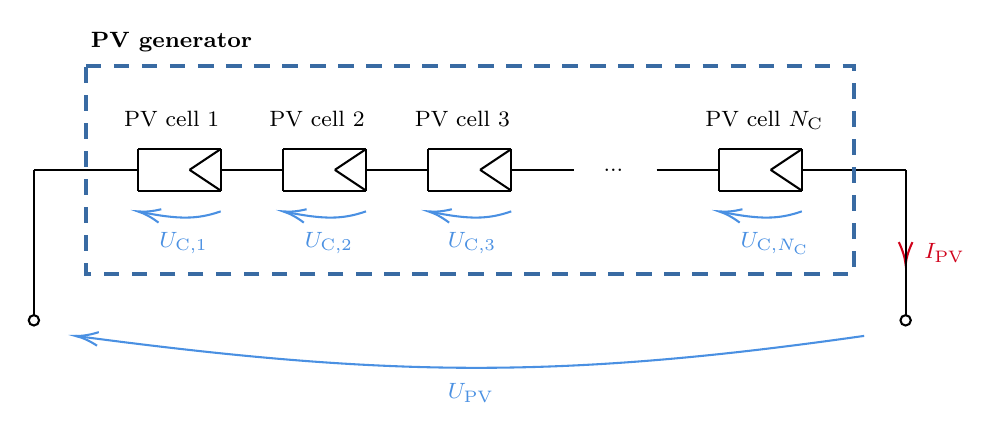
\begin{tikzpicture}[x=0.75pt,y=0.75pt,yscale=-1,xscale=1]
%uncomment if require: \path (0,300); %set diagram left start at 0, and has height of 300

%Straight Lines [id:da607551945482224] 
\draw [color={rgb, 255:red, 208; green, 2; blue, 27 }  ,draw opacity=1 ]   (560,180) -- (560,193.75) ;
\draw [shift={(560,195.75)}, rotate = 270] [color={rgb, 255:red, 208; green, 2; blue, 27 }  ,draw opacity=1 ][line width=0.75]    (10.93,-3.29) .. controls (6.95,-1.4) and (3.31,-0.3) .. (0,0) .. controls (3.31,0.3) and (6.95,1.4) .. (10.93,3.29)   ;
%Straight Lines [id:da39220891738716435] 
\draw    (370,140) -- (370,160) ;
%Straight Lines [id:da26376681003549773] 
\draw    (370,140) -- (355,150) ;
%Straight Lines [id:da7171194033958681] 
\draw    (355,150) -- (370,160) ;
%Straight Lines [id:da7758232590553849] 
\draw    (370,140) -- (330,140) ;
%Straight Lines [id:da23922780724985704] 
\draw    (370,160) -- (330,160) ;
%Straight Lines [id:da8647396746050291] 
\draw    (330,140) -- (330,160) ;
%Shape: Circle [id:dp9465717065223571] 
\draw   (560,220) .. controls (561.38,220) and (562.5,221.12) .. (562.5,222.5) .. controls (562.5,223.88) and (561.38,225) .. (560,225) .. controls (558.62,225) and (557.5,223.88) .. (557.5,222.5) .. controls (557.5,221.12) and (558.62,220) .. (560,220) -- cycle ;
%Straight Lines [id:da8361729954042678] 
\draw    (300,140) -- (300,160) ;
%Straight Lines [id:da8303503310697085] 
\draw    (300,140) -- (285,150) ;
%Straight Lines [id:da6935206293495084] 
\draw    (285,150) -- (300,160) ;
%Straight Lines [id:da4478328338561339] 
\draw    (300,140) -- (260,140) ;
%Straight Lines [id:da6338115192168345] 
\draw    (300,160) -- (260,160) ;
%Straight Lines [id:da4710313866121387] 
\draw    (260,140) -- (260,160) ;
%Straight Lines [id:da04529427678773623] 
\draw    (510,140) -- (510,160) ;
%Straight Lines [id:da12585917694032633] 
\draw    (510,140) -- (495,150) ;
%Straight Lines [id:da5777912998057524] 
\draw    (495,150) -- (510,160) ;
%Straight Lines [id:da8526647582658238] 
\draw    (510,140) -- (470,140) ;
%Straight Lines [id:da18181567227521733] 
\draw    (510,160) -- (470,160) ;
%Straight Lines [id:da08821152259447507] 
\draw    (470,140) -- (470,160) ;
%Straight Lines [id:da004318261204414364] 
\draw    (300,150) -- (330,150) ;
%Straight Lines [id:da415576466861697] 
\draw    (440,150) -- (470,150) ;
%Straight Lines [id:da5030082829613725] 
\draw    (230,140) -- (230,160) ;
%Straight Lines [id:da24153450583970604] 
\draw    (230,140) -- (215,150) ;
%Straight Lines [id:da7169826080141817] 
\draw    (215,150) -- (230,160) ;
%Straight Lines [id:da8893075482646204] 
\draw    (230,140) -- (190,140) ;
%Straight Lines [id:da8414185658377555] 
\draw    (230,160) -- (190,160) ;
%Straight Lines [id:da030501270201809483] 
\draw    (190,140) -- (190,160) ;
%Straight Lines [id:da11000547395248828] 
\draw    (140,150) -- (190,150) ;
%Straight Lines [id:da8573962154803463] 
\draw    (230,150) -- (260,150) ;
%Straight Lines [id:da9793828451968309] 
\draw    (370,150) -- (400,150) ;
%Straight Lines [id:da6281863128480734] 
\draw    (510,150) -- (560,150) ;
%Shape: Rectangle [id:dp583588773515656] 
\draw  [color={rgb, 255:red, 57; green, 107; blue, 163 }  ,draw opacity=1 ][dash pattern={on 5.63pt off 4.5pt}][line width=1.5]  (165,100) -- (535,100) -- (535,200) -- (165,200) -- cycle ;
%Curve Lines [id:da418839437477464] 
\draw [color={rgb, 255:red, 74; green, 144; blue, 226 }  ,draw opacity=1 ]   (230,170) .. controls (218.85,173.88) and (210.04,174) .. (191.73,170.35) ;
\draw [shift={(190,170)}, rotate = 371.59000000000003] [color={rgb, 255:red, 74; green, 144; blue, 226 }  ,draw opacity=1 ][line width=0.75]    (10.93,-3.29) .. controls (6.95,-1.4) and (3.31,-0.3) .. (0,0) .. controls (3.31,0.3) and (6.95,1.4) .. (10.93,3.29)   ;
%Curve Lines [id:da498717897550782] 
\draw [color={rgb, 255:red, 74; green, 144; blue, 226 }  ,draw opacity=1 ]   (300,170) .. controls (288.84,173.88) and (280.04,174) .. (261.73,170.35) ;
\draw [shift={(260,170)}, rotate = 371.59000000000003] [color={rgb, 255:red, 74; green, 144; blue, 226 }  ,draw opacity=1 ][line width=0.75]    (10.93,-3.29) .. controls (6.95,-1.4) and (3.31,-0.3) .. (0,0) .. controls (3.31,0.3) and (6.95,1.4) .. (10.93,3.29)   ;
%Curve Lines [id:da08475302030352005] 
\draw [color={rgb, 255:red, 74; green, 144; blue, 226 }  ,draw opacity=1 ]   (370,170) .. controls (358.85,173.88) and (350.04,174) .. (331.73,170.35) ;
\draw [shift={(330,170)}, rotate = 371.59000000000003] [color={rgb, 255:red, 74; green, 144; blue, 226 }  ,draw opacity=1 ][line width=0.75]    (10.93,-3.29) .. controls (6.95,-1.4) and (3.31,-0.3) .. (0,0) .. controls (3.31,0.3) and (6.95,1.4) .. (10.93,3.29)   ;
%Curve Lines [id:da12741622664998054] 
\draw [color={rgb, 255:red, 74; green, 144; blue, 226 }  ,draw opacity=1 ]   (510,170) .. controls (498.85,173.88) and (490.04,174) .. (471.73,170.35) ;
\draw [shift={(470,170)}, rotate = 371.59000000000003] [color={rgb, 255:red, 74; green, 144; blue, 226 }  ,draw opacity=1 ][line width=0.75]    (10.93,-3.29) .. controls (6.95,-1.4) and (3.31,-0.3) .. (0,0) .. controls (3.31,0.3) and (6.95,1.4) .. (10.93,3.29)   ;
%Straight Lines [id:da46920157249938654] 
\draw    (560,150) -- (560,220) ;
%Shape: Circle [id:dp649544243274581] 
\draw   (140,220) .. controls (141.38,220) and (142.5,221.12) .. (142.5,222.5) .. controls (142.5,223.88) and (141.38,225) .. (140,225) .. controls (138.62,225) and (137.5,223.88) .. (137.5,222.5) .. controls (137.5,221.12) and (138.62,220) .. (140,220) -- cycle ;
%Straight Lines [id:da23605717922255787] 
\draw    (140,150) -- (140,220) ;
%Curve Lines [id:da371666183196145] 
\draw [color={rgb, 255:red, 74; green, 144; blue, 226 }  ,draw opacity=1 ]   (540,230) .. controls (392.5,251) and (310.5,250) .. (160,230) ;
\draw [shift={(160,230)}, rotate = 367.57] [color={rgb, 255:red, 74; green, 144; blue, 226 }  ,draw opacity=1 ][line width=0.75]    (10.93,-3.29) .. controls (6.95,-1.4) and (3.31,-0.3) .. (0,0) .. controls (3.31,0.3) and (6.95,1.4) .. (10.93,3.29)   ;

% Text Node
\draw (182,120) node [anchor=north west][inner sep=0.75pt]  [font=\footnotesize] [align=left] {PV cell $\displaystyle 1$};
% Text Node
\draw (567.5,183.9) node [anchor=north west][inner sep=0.75pt]  [font=\footnotesize,color={rgb, 255:red, 208; green, 2; blue, 27 }  ,opacity=1 ]  {$I_{\mathrm{PV}}$};
% Text Node
\draw (199,178.4) node [anchor=north west][inner sep=0.75pt]  [font=\footnotesize,color={rgb, 255:red, 74; green, 144; blue, 226 }  ,opacity=1 ]  {$U_{\mathrm{C,} 1}$};
% Text Node
\draw (269,178.4) node [anchor=north west][inner sep=0.75pt]  [font=\footnotesize,color={rgb, 255:red, 74; green, 144; blue, 226 }  ,opacity=1 ]  {$U_{\mathrm{C} ,2}$};
% Text Node
\draw (338,178.4) node [anchor=north west][inner sep=0.75pt]  [font=\footnotesize,color={rgb, 255:red, 74; green, 144; blue, 226 }  ,opacity=1 ]  {$U_{\mathrm{C} ,3}$};
% Text Node
\draw (479,178.4) node [anchor=north west][inner sep=0.75pt]  [font=\footnotesize,color={rgb, 255:red, 74; green, 144; blue, 226 }  ,opacity=1 ]  {$U_{\mathrm{C} ,N_{\mathrm{C}}}$};
% Text Node
\draw (252,120) node [anchor=north west][inner sep=0.75pt]  [font=\footnotesize] [align=left] {PV cell $\displaystyle 2$};
% Text Node
\draw (322,120) node [anchor=north west][inner sep=0.75pt]  [font=\footnotesize] [align=left] {PV cell $\displaystyle 3$};
% Text Node
\draw (462,120) node [anchor=north west][inner sep=0.75pt]  [font=\footnotesize] [align=left] {PV cell $\displaystyle N_{\mathrm{C}}$};
% Text Node
\draw (338,251.4) node [anchor=north west][inner sep=0.75pt]  [font=\footnotesize,color={rgb, 255:red, 74; green, 144; blue, 226 }  ,opacity=1 ]  {$U_{\mathrm{PV}}$};
% Text Node
\draw (413,148) node [anchor=north west][inner sep=0.75pt]  [font=\footnotesize] [align=left] {...};
% Text Node
\draw (166,82) node [anchor=north west][inner sep=0.75pt]  [font=\footnotesize] [align=left] {\textbf{PV generator}};


\end{tikzpicture}
